\documentclass{article}
\usepackage{fullpage}
\usepackage{amsmath,amssymb,amsfonts}
\usepackage{graphicx}
\usepackage{natbib}
\usepackage[colorinlistoftodos]{todonotes}


\def\R{{\mathbb{R}}}
\def\pr{{\rm Pr}}
\def\E{{\mathbb E}}
\def\X{{\mathcal X}}
\def\Y{{\mathcal Y}}
\def\H{{\mathcal H}}
\def\G{{\mathcal G}}
\def\B{{\mathcal B}}
\def\yh{{\widehat{y}}}
\def\bias{{\rm bias}}
\def\supp{{\rm supp}}
\def\sign{{\rm sign}}
\def\PL{{\mbox{\rm PL}}}

\newtheorem{thm}{Theorem}
\newtheorem{lemma}[thm]{Lemma}
\newtheorem{cor}[thm]{Corollary}
\newtheorem{claim}[thm]{Claim}
\newtheorem{defn}[thm]{Definition}
\newtheorem{assump}{Assumption}
\newtheorem{open}{Open problem}
\newenvironment{proof}{\noindent {\sc Proof:}}{$\Box$ \medskip}

\newcommand{\comment}[3]{{\color{#1} {\bf #2 :} #3}}
%\newcommand{\comment}[3]{}  % suppress comments
\newcommand{\yoav}[1]{\comment{cyan}{Yoav}{#1}}
\newcommand{\sanjoy}[1]{\comment{blue}{Sanjoy}{#1}}

\DeclareMathOperator*{\argmax}{arg\,max}

\title{Active learning using region-based sampling}

\begin{document}

\maketitle

\section{Setup}

\begin{itemize}
\item {\it Underlying model of data.}

\begin{itemize}
\item Instances lie in a metric space $(\X, d)$. 
\item Label space $\Y = \{-1,+1\}$. Each $x \in \X$ is labeled according to an unknown conditional probability function $\Pr(Y|X)$, with
$$ \eta(x) = \E[Y | X=x] = \pr(Y=1|X=x) - \pr(Y=-1|X=x) = 2 \pr(Y=1|X=x) - 1 .$$
\item The {\it Bayes-optimal classifier} on $\X$ is $g^*(x) = \sign(\eta(x))$.
\end{itemize}

\item {\it Task: Finite population labeling.}

\begin{itemize}
\item We are given a finite dataset $X \subset \X$ of $n$ points, and have the ability to query the labels of any of them. We are also given parameters $0 < \gamma, \delta < 1$.
\item We want a procedure that chooses the next point, or batch of points, to query. This process will be applied repeatedly and then stopped at an arbitrary time, whereupon labels $\yh(x)$ must be provided for all $x \in X$ (including those that were queried).
\item We would like the inferred labels $\yh(x)$ to approach the Bayes-optimal labels $g^*(x)$ as quickly as possible, ideally much faster than would occur if the query points were chosen uniformly at random.
\item Specifically, we are judged on the number of errors on points $x \in X$ with $|\eta(x)| > \gamma$:
$$ \sum_{x \in X} {\bf 1}(\yh(x) \neq g^*(x),\ |\eta(x)| > \gamma) .$$
The procedure is allowed to fail with probability $\delta$, to account for sampling error.
\end{itemize}

\end{itemize}

\section{Active learning algorithm}

\subsection{Some details}

\begin{enumerate}

\item {\it Sampling regions.}
The sampling is organized around a collection $\B$ of measurable subsets of $\X$. These are the atomic sets on which we assess label bias and we call them ``balls''.

\begin{enumerate}

\item[(a)] {\it Points within a ball.} For any ball $B \in \B$, let $X_B = X \cap B$ denote the points in $X$ that will be used to assess the bias of $B$.\footnote{Sometimes, $\B$ might be constructed in a way that depends on $X$ and causes certain points to be excluded. For instance, consider these two alternatives for defining $\B$:
\begin{itemize}
\item $\B$ consists of a pre-defined set of balls.
\item $\B$ consists of balls defined by pairs of points in $X$, with each $x,x' \in X$ yielding the ball $B(x,\|x-x'\|)$.
\end{itemize}
In the first case, all points $X \cap B$ are random draws from $B$. In the second case, this is also true except for the two points $x,x'$ that define the ball.}

\item[(b)] {\it Grouping balls by size.} We will group balls by the number of points that they contain: we put $B$ at {\it level} $\ell$ if
$$ \frac{n}{2^{\ell + 1}} \leq |X_B| < \frac{n}{2^\ell} .$$
Here $\ell$ ranges from $0$ (consisting of balls that contain at least half the data points) to roughly $\lg n$ (containing a single point). 

Let $\B_\ell$ consist of all balls in $\B$ that are at level $\ell$. Thus $\B_0, \B_1, \ldots$ is a partition of $\B$, with $\B_0$ consisting of very large balls and subsequent $\B_1, \B_2, \ldots$ consisting of successively smaller balls.

\item[(c)] {\it Balls used to evaluate a given point.}

For any $x \in \X$, let $\B(x) \subset \B$ denote the collection of balls that will be used in determining $x$'s label. We will take these to be all balls that contain $x$. As before, we can partition these balls by sampling-level, so that $\B_\ell(x) = \B(x) \cap \B_\ell$.

\end{enumerate}

\item {\it Bias-estimates for balls and for data points.} The active learning algorithm uses label-queries to assess the bias of balls $B \in \B$. In turn, these are used to estimate the labels of individual points.

\begin{enumerate}

\item[(a)] {\it Bias of a ball.} The bias of a ball $B \in \B$ is defined as
$$ \eta_X(B) = \mbox{average}\{\eta(x): x \in X_B \} .$$

\item[(b)] {\it Qualitative estimates of bias.} Each ball $B$ is assigned qualitative bias estimate,
$$ \yh(B) = 
\left\{
\begin{array}{cl}
+1 & \mbox{significant $+$ bias} \\
-1 & \mbox{significant $-$ bias} \\
0 & \mbox{no significant bias} \\
\bot & \mbox{not yet available}
\end{array}
\right.
$$
The option $\bot$ is used until sufficiently many points in $X_B$ have been labeled: the required number, $k$, is roughly $1/\gamma^2$ (recall that $\gamma$ is the smallest bias that needs to be detected). Once this many labels are available, $\yh(B)$ is set to a value in $\{-1,0,+1\}$ and remains fixed thereafter.

\item[(c)] {\it Bias guarantees.} Our bias estimates will satisfy a guarantee of the following form: with probability $1-\delta$, for all $B \in \B$, once $\yh(B)$ is set to a value in $\{-1,0,+1\}$, 
\begin{itemize}
\item $\yh(B) = +1 \implies \eta_X(B) > b_1$
\item $\yh(B) = -1 \implies \eta_X(B) < -b_1$
\item $\yh(B) = 0 \implies |\eta_X(B)| < b_2$
\end{itemize}
for some constants $0 < b_1 < b_2 < 1$.

\item[(d)] {\it supported labels for a point.} Pick an instance $x$ and a level $\ell$. We say that a ball $B \in \B_\ell(x)$ {\em supports} the label $s \in \{-1,+1\}$ if $\yh(B) = s$. The set of {\em supported labels} for $x$ at level $\ell$ is defined as:
\begin{equation}
\PL_\ell(x) = \{s \in \{-1, +1\}: \mbox{there exists $B \in \B_\ell(x)$ with $\yh(B) = s$} \} 
\label{eq:PL}
\end{equation}

\item[(e)] {\it The label of a point at level $\ell$.} The label of point $x$ at level $\ell$ is a value $\yh_\ell(x) \in \{-1,+1,0,!,\bot\}$. It is initially $\bot$ (meaning ``not yet available''), but once bias-estimates are available for all $B \in \B_\ell(x)$, it is set to a value in $\{-1,+1,0,!\}$ and remains fixed thereafter:
\begin{equation}
\yh_\ell(x) = 
\left\{
\begin{array}{cl}
+1 & \mbox{if $\PL_\ell(x) = \{+1\}$} \\
-1 &  \mbox{if $\PL_\ell(x) = \{-1\}$} \\
0 & \mbox{if $\PL_\ell(x) = \{\}$} \\
! & \mbox{if $\PL_\ell(x) = \{-1,+1\}$}
\end{array}
\right.
\label{eq:provisional-label}
\end{equation}
\end{enumerate}
\end{enumerate}

It is worth noting that, while non-parametric methods, of the type described here are guaranteed to converge to the Bayes optimal classifier, the algorithm never knows whether the label on any point $x \in \X$ has converged. We say that our algorithm had a {\em mind change} on $x$ if $\yh_\ell(x)=+1$ and $\yh_{\ell+1}=-1$ or vice versa. It is not hard to construct cases where the number of mind changes for a point $x$ is arbitrarily large. 

In other words the algorithm never knows what is the Bayes optimal label of any point. We divide the points into those labeled $!$ which are the {\em known unknowns} and all of the other points which are the {\em unknown unknowns}.
The basic idea of our algorithm is to focus half of its queries on the known unknowns, and the other half  querying all instances.

\subsection{The algorithm}

The overall active learning algorithm is in Figure~\ref{alg:main}. It makes calls to subroutines for background and focused sampling, shown in Figure~\ref{alg:sampling}. The querying process can be stopped at any time, whereupon labels will be assigned as follows:
\begin{equation}
\yh(x) = 
\left\{
\begin{array}{ll}
\yh_\ell(x) & \mbox{for the largest $\ell$ with $\yh_\ell(x) \in \{-1,+1\}$, if such an $\ell$ exists} \\
0 & \mbox{(don't know), otherwise}
\end{array}
\right.
\label{eq:final-label}
\end{equation}

\begin{figure}[h!]
\framebox{
\begin{minipage}[t]{6.4in}
\begin{itemize}
\item Initialize uncertainty regions at all levels:
\begin{itemize}
\item $U_0 = X$
\item $U_\ell = \emptyset$ for $\ell \geq 1$
\end{itemize}
\item Initialize labels at all levels to ``unavailable'':
\begin{itemize}
\item $\yh_\ell(x) = \bot$ for all $x$ and $\ell \geq 0$
\end{itemize}
\item Repeat:
\begin{itemize}
\item If there is a level $\ell \geq 0$ such that $U_\ell \neq \emptyset$:
\begin{itemize}
\item Let $\ell'$ be the smallest such level
\item {\tt Focused-query}($\ell', U_{\ell'}$)
\end{itemize}
\item {\tt Background-query}
\item Update labels:
\begin{itemize}
\item Get bias-estimate $\yh(B) \in \{-1,0,+1\}$ for all $B \in \B$ that are now adequately sampled
\item For each $x \in X$ and level $\ell \geq 0$ for which all of $\B_\ell(x)$ is now sampled:
\begin{itemize}
\item Determine the possible labels for $x$ at level $\ell$:
$$\PL_\ell(x) = \{s \in \{-1, +1\}: \mbox{there exists $B \in \B_\ell(x)$ with $\yh(B) = s$} \}$$
\item Set
$$
\yh_\ell(x) = 
\left\{
\begin{array}{cl}
+1 & \mbox{if $\PL_\ell(x) = \{+1\}$} \\
-1 &  \mbox{if $\PL_\ell(x) = \{-1\}$} \\
0 & \mbox{if $\PL_\ell(x) = \{\}$} \\
! & \mbox{if $\PL_\ell(x) = \{-1,+1\}$}
\end{array}
\right.
$$
\end{itemize}
\end{itemize}
\item Update uncertainty regions:
\begin{itemize}
\item $U_0 = \{x \in X: \yh_0(x) = \bot\}$
\item For all levels $\ell \geq 1$: $U_\ell = \{x \in X: \yh_{\ell-1}(x) = \,!, \ \yh_\ell(x) = \bot\}$
\end{itemize}
\end{itemize}

\end{itemize}

\end{minipage}}
\caption{The active learning algorithm. Each iteration of the main loop makes (at most) one focused query and one background query. The subroutines {\tt Focused-query} and {\tt Background-query} appear in Figure~\ref{alg:sampling}.}
\label{alg:main}
\end{figure}


\begin{figure}[h!]
\framebox{
\begin{minipage}[t]{6.4in}

\vspace{.1in}
\emph{Initialization:}
\begin{itemize}
\item Set $Q = \emptyset$ (points queried so far)
\item For each $x \in X$: choose $T_x \sim \mbox{uniform}([0,1])$
\end{itemize}

\vspace{.2in}
{\bf Focused-query}($\ell, U$)

\vspace{.1in}
\begin{itemize}
\item Define querying region:
$$ S =  \bigcup_{x \in U} \bigcup_{B \in \B_\ell(x)} \{z \in X_B: T_z \leq \tau_\ell\} $$
\item Query the next unlabeled point in $S \setminus Q$, ordered by $T_z$ values, and add to $Q$
\end{itemize}

\vspace{.2in}
{\bf Background-query}

\vspace{.1in}
\begin{itemize}
\item Query the next unlabeled point in $X \setminus Q$, ordered by $T_z$ values, and add to $Q$
\end{itemize}

\end{minipage}}
\caption{The sampling procedures. Each point $x \in X$ has an associated value $T_x$ chosen uniformly at random from $[0,1]$. This smaller this value, the earlier this point is likely to be queried. The focused querying procedure uses level-based thresholds $\tau_\ell = \min(2^{\ell+2}k/n, 1)$.} 
\label{alg:sampling}
\end{figure}


\section{Analysis of algorithm: finite population setting}

We now analyze the active learning procedure for the finite population annotation problem introduced earlier.

\subsection{Accuracy of bias estimates}

We'll start with a uniform guarantee on the bias estimates for all balls $B \in \B$.

Recall that each point $x \in X$ gets a label $Y \in \{-1,+1\}$ according to the distribution
$$ \eta(x) = \E[Y | X=x].$$ 
For any $B \in \B$ with $X_B \neq \emptyset$, let $\eta_X(B)$ be the average $\eta$-value of the points in $B$, that is,
$$ \eta_X(B) = \frac{1}{|X_B|} \sum_{x \in X_B} \eta(x) .$$
The specific property we need is encapsulated in the following definition.

\yoav{I think instead of this definition it would be  better to point to item (c) "Bias estimatess ..."}
\begin{defn}
For any $B \in \B$ and $0 < b_1 < b_2$, we say bias estimate $\yh(B) \in \{+1,-1,0\}$ is \emph{$(b_1,b_2)$-accurate} if the following holds:
\begin{itemize}
\item $\yh(B) = +1 \implies \eta_X(B) > b_1$
\item $\yh(B) = -1 \implies \eta_X(B) < -b_1$
\item $\yh(B) = 0 \implies |\eta_X(B)| < b_2$
\end{itemize}
\label{def:accurate-bias-estimate}
\end{defn}
For reference, we will take $b_1 = \gamma/2$ and $b_2 = \gamma$, where $\gamma$ is the minimum bias we need to detect, as per the problem specification.

In what follows, take $0 < \delta < 1$ to be a predefined constant, and define
\begin{equation}
c_1 = \sqrt{3 \ln \frac{4|\B|}{\delta}} .
\label{eq:c1}
\end{equation}

For any level $\ell$, define threshold $\tau_\ell$ as follows:
\begin{equation}
\tau_\ell = \min \left( \frac{2^{\ell+2}k}{n}, \ 1 \right)
\label{eq:threshold-ell}
\end{equation}
\yoav{What is $k$? Oh, I think it is the minimal number of queries to identify a bias $\gamma$,... not sure where it is defined.}

For any $B \in \B_\ell$, define its \emph{query-set} to be $\Gamma(B) = \{z \in X_B: T_z \leq \tau_\ell\}$. We base our bias-estimate for $B$ on the labels of points in $\Gamma(B)$.

Our main deviation bound is the following, a consequence of Lemma~\ref{lemma:large-deviation-discrete} in the appendix.
\begin{thm}[checked]
Suppose $k \geq 2c_1^2$. With probability at least $1-\delta$, the following is true for all $B \in \B$ with $|X_B| \geq k$:
\begin{enumerate}
\item[(a)] The query set $\Gamma(B)$ has size at least $k$.
\item[(b)] The average label on $\Gamma(B)$, call it $\widehat{\eta}(B)$, satisfies
$$ \left| \widehat{\eta}(B) - \eta_X(B) \right| \leq \frac{4c_1}{\sqrt{k}}.$$
\end{enumerate}
\label{thm:large-deviation-bounds}
\end{thm}
\begin{proof}
These follow immediately by applying Lemma~\ref{lemma:large-deviation-discrete} to each $B \in \B$ and taking a union bound. In particular, note that the choice of $\tau_\ell$ ensures $|X_B| \tau_\ell \geq 2k$.
\end{proof}

The following corollary of Theorem~\ref{thm:large-deviation-bounds} is immediate.
\begin{cor}[checked]
Suppose that $k \geq (8c_1/(b_2-b_1))^2$ where $c_1$ is given in (\ref{eq:c1}). 
For each $B \in \B$, let $\widehat{\eta}(B)$ be the average label on the query-set $\Gamma(B)$, and define the bias-estimate $\yh(B)$ as follows:
$$ \yh(B)
= 
\left\{
\begin{array}{ll}
\sign(\widehat{\eta}(B)) & \mbox{if $|\widehat{\eta}(B)| \geq (b_1 + b_2)/2$} \\
0 & \mbox{otherwise}
\end{array}
\right.
$$
With probability $\geq 1-\delta$, all bias estimates $\yh(B)$, for $B \in \B$, are $(b_1,b_2)$-accurate.
\label{cor:accurate-bias-estimates}
\end{cor}
\begin{proof}
By the choice of $k$, we have from Theorem~\ref{thm:large-deviation-bounds} that 
$$ \left| \widehat{\eta}(B) - \eta_X(B) \right| < \frac{b_2 - b_1}{2} $$
for all $B \in \B$.
\end{proof}

In what follows, we will assume that this $(1-\delta)$-probability event holds.

\subsection{Mind changes}

The label assigned to a data point $x$ at level $\ell$, which we denote $\yh_\ell(x)$, might change as $\ell$ increases; it may flip between $+1$ and $-1$ a few times, with stretches of $0$ or $!$ in between.

We distinguish two critical levels for each $x$: the level $L_s(x)$ by which $\yh_\ell(x)$ has ``stabilized'' in the sense that it no longer flips between $+1$ and $-1$ (although it may be $!$), and the level $L_f(x)$ by which $\yh_\ell(x)$ is correct and thus ``finalized''. See Figure~\ref{fig:two-levels} for a pictorial view.

\begin{figure}
\begin{center}
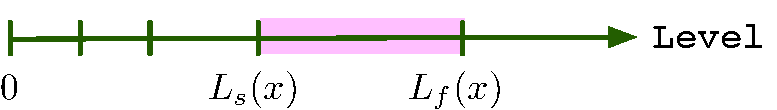
\includegraphics[width=3.5in]{home-stretch.pdf}
\end{center}
\caption{The tentative label $\yh_\ell(x)$ of a given point $x$ can undergo several mind-changes as the neighborhood of $x$ is sampled at successively finer levels. Beyond level $L_s(x)$, this $\yh_\ell(x)$ will never be the wrong label, but might be $!$. Beyond level $L_f(x)$, the correct label will be assigned.}
\label{fig:two-levels}
\end{figure}

\begin{defn}
Pick any $x \in X$ with $\eta(x) \neq 0$ and let $g^*(x) = \sign(\eta(x))$ be its Bayes-optimal label. We define $L_s(x)$ to be the smallest integer such that for all $\ell \geq L_s(x)$, the following condition holds:
\begin{enumerate}
\item[1.] Some $B \in \B_\ell(x)$ has $g^*(x) \cdot \eta_X(B) \geq b_2$.
\end{enumerate}
(If there is no such level, we define $L_s(x) = \infty$.) We define $L_f(x)$ to be the smallest integer such that for all $\ell \geq L_f(x)$, the above condition holds, and additionally:
\begin{enumerate}
\item[2.] Every $B \in \B_\ell(x)$ has $g^*(x) \cdot \eta_X(B) \geq -b_1$.
\end{enumerate} 
(Again, take $L_f(x) = \infty$ if there is no such level.) 
\label{defn:Lsf}
\end{defn}
Condition 1 says that there is a good neighborhood $B \in \B_\ell(x)$, one with a strong bias towards the correct label of $x$. Condition 2 says that there are no bad neighborhoods, that are weakly biased towards the wrong label.

Thus $L_s(x) \leq L_f(x)$, and there might be a large gap between the two. Before the background sampling reaches level $L_s(x)$, it is quite possible that we will predict the wrong label for $x$. However, once all balls in $\B_{L_s(x)}(x)$ have been adequately sampled, point $x$ will either (i) be assigned label $!$ and put in the uncertainty set, in which case it will benefit from focused sampling, or (ii) will get the correct label. Once the balls in $\B_{L_f(x)}(x)$ have been sampled, condition (ii) will hold.

\begin{lemma}[checked]
Pick any $x \in X$ with $\eta(x) \neq 0$ and let $g^*(x) \in \{+1,-1\}$ denote its Bayes-optimal label. Then for any level $\ell$ and any time at which $\yh_\ell(x) \neq \bot$:
\begin{enumerate}
\item[(a)] If $\ell \geq L_s(x)$, then $\yh_\ell(x) \in \{g^*(x), !\}$.
\item[(b)] If $\ell \geq L_f(x)$, then $\yh_\ell(x) = g^*(x)$.
\end{enumerate}
\label{lemma:boundary}
\end{lemma}
\begin{proof}
For part (a), note that if $\ell \geq L_s(x)$, then some $B \in \B_\ell(x)$ has significant bias towards the correct label $g^*(x)$, in which case (by Corollary~\ref{cor:accurate-bias-estimates}) $\yh(B) = g^*(x)$. Thus $\yh_\ell(x)$ must either be $!$ (if there is some $B' \in \B_\ell(x)$ with $\yh(B') = -g^*(x)$) or $g^*(x)$.

For (b), both conditions (1) and (2) of Definition~\ref{defn:Lsf} hold, so there is at least one $B \in \B_\ell(x)$ with $\yh(B) = g^*(x)$ and no $B$ with $\yh(B) = -g^*(x)$. Thus $\yh_\ell(x) = g^*(x)$.
\end{proof}

\subsection{Bounding the amount of focused sampling}

From Lemma~\ref{lemma:boundary}(b), we see that the label of a point $x$ will be apparent by the time it has been sampled at level $L_f(x)$, and thus $x$ will not appear in the uncertainty set for subsequent levels. That is, 
$$U_{\ell} \subset \{x \in X: L_f(x) \geq \ell\}.$$ 
This in turns gives a simple characterization of the points that are queried as part of focused sampling.
\begin{lemma}[checked]
All focused samples at level $\ell$ lie in $\{z \in \Delta_\ell: T_z \leq \tau_\ell \}$, where
\begin{equation}
\Delta_\ell 
= \bigcup_{x \in X: L_f(x) \geq \ell} \bigcup_{B \in \B_{\ell}(x)} X_B 
.
\label{eq:sampling-region}
\end{equation}
\label{lemma:focused}
\end{lemma}
\begin{proof}
Let $\overline{U}_\ell$ denote the set of all points that are ever (in any round of sampling) in the uncertainty set at level $\ell$. As is apparent from the {\tt Focused-query} subroutine (Figure~\ref{alg:sampling}), all focused samples at level $\ell$ lie in
$$
\bigcup_{x \in \overline{U}_\ell} \bigcup_{B \in \B_\ell(x)} \{z \in X_B: T_z \leq \tau_\ell \}
\ 
\subset 
\ 
\bigcup_{x \in X: L_f(x) \geq \ell} \bigcup_{B \in \B_\ell(x)} \{z \in X_B: T_z \leq \tau_\ell \}
\ 
=
\ 
\{z \in \Delta_\ell: T_z \leq \tau_\ell \},
$$
where the first containment is a consequence of Lemma~\ref{lemma:boundary}.
\end{proof}


A final property we will need for label complexity bounds is that various subsets of interest contain roughly the expected number of points at each level.
\begin{lemma}
Pick any $0 < \ell_o \leq \lg n$. With probability at least $1-2(\ell_o+1)e^{-k/3}$, the following hold for all levels $0 \leq \ell \leq \ell_o$.
\begin{enumerate}
\item[(a)] $|\{x \in X: T_x \leq \tau_\ell\}| < 2 n \tau_\ell$.
\item[(b)] If $|\Delta_\ell| \tau_\ell \geq k$ then $|\{x \in \Delta_{\ell}: T_x \leq \tau_\ell\}| < 2 |\Delta_\ell| \tau_\ell$.
\end{enumerate}
\label{lemma:level-distribution}
\end{lemma}
\begin{proof} 
Pick any subset $S \subset X$ and let $m = |S|$. Then $|\{x \in S: T_x \leq \tau_\ell\}|$ has a $\mbox{binomial}(m, \tau_\ell)$ distribution with expectation $m \tau_\ell$. The probability that it is greater than or equal to twice its expected value is, by a multiplicative Chernoff bound, at most $e^{-m \tau_{\ell}/3}$.

Both parts follow from this principle; and we take a union bound over all $\ell_o + 1$ levels.
\end{proof}

Henceforth we assume that these two bounds hold.

\subsection{Label complexity bounds} 

\begin{thm}
Suppose the active learning algorithm is allowed to make $0 < m \leq n$ queries. Define
$$ \ell_1 = \left\lfloor \lg \frac{m}{32k} \right\rfloor .$$
and let $\ell_2$ be the largest integer such that
$$ \sum_{\ell = \ell_1 + 1}^{\ell_2} |\Delta_{\ell}| \, \tau_\ell \ \leq \ \frac{m}{8} .$$
Then any point $x \in X$ with $L_s(x) \leq \ell_1$ and $L_f(x) \leq \ell_2$ will have final label $\yh(x) = g^*(x)$.
\label{thm:label-complexity}
\end{thm}
\begin{proof}
Denote the first $m/2$ queries by {\it phase one} and the second $m/2$ by {\it phase two}. We will analyze the effect of background sampling in phase one and focused sampling in phase two. We start with the former.

Of the $m/2$ queries in phase one, at least $m/4$ will be background samples. Therefore the $m/4$ points with lowest $T_x$ values are guaranteed to be queried.

Now, for $\ell_1$ as defined, we have from (\ref{eq:threshold-ell}) that $\tau_{\ell_1} \leq m/8n$ and thus from Lemma~\ref{lemma:level-distribution}(a) that at most $m/4$ points in $X$ satisfy $T_x \leq \tau_{\ell_1}$. Therefore all such points are queried in phase one, and all label-estimates $\{\yh_{\ell_1}(x): x \in X\}$ are set.

It then follows from Lemma~\ref{lemma:boundary} that the following hold for any $x \in X$ with $L_s(x) \leq \ell_1$:
\begin{enumerate}
\item[(a)] By the end of phase one, $\yh_{\ell_1}(x) \in \{g^*(x), !\}$.
\item[(b)] For any $\ell > \ell_1$, when $\yh_\ell(x)$ becomes available, it lies in $\{g^*(x), !\}$.
\item[(c)] If $x$ ever leaves the combined uncertainty region $U = \cup_\ell U_\ell$ during phase two, then its final label as defined in (\ref{eq:final-label}) is henceforth always $\yh(x) = g^*(x)$.
\end{enumerate}

Now let's move on to phase two. Let $A = \{x \in X: L_s(x) \leq \ell_1, L_f(x) \leq \ell_2\}$. We will show that every point in $A$ must leave the uncertainty region $U$ at some time during phase two. From (c), we can conclude that all these points have their final labels set correctly, once and for all.

We will break the argument into two cases. 

{\it Case 1:} Fewer than $m/4$ focused queries are made in phase two. This can only happen if some round of sampling has an empty uncertainty set, meaning that all of $A$ has left $U$ at that point.

{\it Case 2:} A full $m/4$ focused queries are made in phase two. By the analysis of phase one, none of these queries can be at level $\leq \ell_1$ and by Lemma~\ref{lemma:focused}, the total number of possible focused queries at levels $\ell_1+1$ through $\ell_2$ inclusive is at most
$$\sum_{\ell=\ell_1+1}^{\ell_2} |\{z \in \Delta_{\ell}: T_z \leq \tau_\ell \}| 
\ < \ 
\sum_{\ell=\ell_1+1}^{\ell_2} 2 |\Delta_{\ell}| \tau_\ell
\ \leq \ 
\frac{m}{4} ,
$$
where the first inequality is from Lemma~\ref{lemma:level-distribution}(b). Thus at least one query in phase two must be at level $\ell_2 +1$. When this query is made, every $U_\ell$ with $\ell \leq \ell_2$ must be empty and thus all of $A$ must have left the uncertainty region (no $x \in A$ can be part of $U_\ell$ for $\ell > \ell_2 \geq L_f(x)$). 

Thus every $x \in A$ must leave the uncertainty region at some point in phase two, and their final labels are subsequently set correctly.
\end{proof}

\subsection{Example: One-dimensional data with Massart noise}

In order to apply Theorem~\ref{thm:label-complexity}, we need
\begin{itemize}
\item upper bounds on the critical levels $L_s(x)$ and $L_f(x)$ for each point $x \in X$, and
\item upper bounds on the size of the sampling region $\Delta_\ell$ at each level $\ell$.
\end{itemize}
We now illustrate how this works out in a canonical setting.

Suppose $X$ is an arbitrary set of $n$ points in $\X = [0,1]$ and is labeled according to a conditional probability function $\eta: \X \to [-1,1]$ that satisfies the Massart noise condition:
\begin{itemize}
\item There are $p$ disjoint open intervals $I_1, \ldots, I_p$, such that $\X$ is (the closure of) their union, and
\item for each $j$, either $\eta(x) > \gamma$ for all $x \in I_j$ or $\eta(x) < -\gamma$ for all $x \in I_j$. In the first case, we write $g^*(I_j) = +1$ and in the second case, $g^*(I_j) = -1$.
\end{itemize}
Here $0 < \gamma < 1$ is some constant. See Figure~\ref{fig:oned-massart} for an illustrative example.

\begin{figure}
\begin{center}
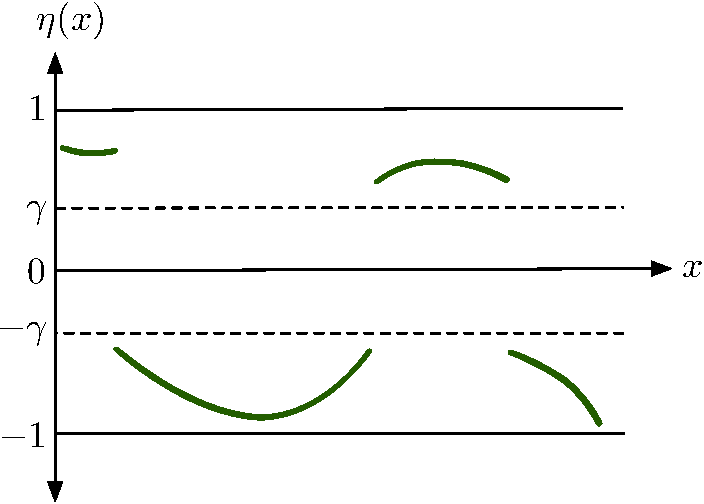
\includegraphics[width=3in]{oned-massart.pdf}
\end{center}
\caption{In this example the conditional probability function $\eta$ is defined by four intervals; on each, $\eta$ is either $> \gamma$ or $<-\gamma$.}
\label{fig:oned-massart}
\end{figure}

We will take $\B$ to consist of all open intervals of $[0,1]$, with $\B(x)$ denoting intervals that contain point $x$. We will choose accuracy parameters $b_1, b_2$ so that $0 < b_1 < b_2 \leq \gamma$.

The intervals $I_j$ can be written in the form $(\lambda_{j-1}, \lambda_j)$, where
$$ 0 = \lambda_0 < \lambda_1 < \lambda_2 < \cdots < \lambda_{p-1} < \lambda_p = 1 .$$
Here $\lambda_1, \ldots, \lambda_{p-1}$ are the \emph{boundary points} between intervals.
\begin{lemma}
Pick any $x \in \X$; suppose $x \in I_j$.
\begin{enumerate}
\item[(a)] Let $n_j = |X \cap I_j|$. Then $L_s(x) \leq \lg (n/n_j)$.
\item[(b)] Let $r(x)$ be the minimum number of data points that lie between $x$ and a boundary point, counting $x$ as well; this is either the number of points in the left-interval $(\lambda_{j-1},x]$ (if $j > 1$) or the right-interval $[x, \lambda_j)$ (if $j < p$), whichever is smaller. Then $L_f(x) \leq \lg (n/r(x))$.
\end{enumerate}
\label{lemma:oned-massart-Lsf}
\end{lemma}
\begin{proof}
For (a), notice first that $I_j \in \B_{\ell}(x)$ for $\ell = \lceil (\lg n/n_j) - 1 \rceil$. Moreover, $g^*(I_j) \cdot \eta_X(I_j) > \gamma \geq b_2$. Thus $I_j$ belongs to $\B_\ell(x)$ and is strongly biased towards the correct label. For levels $> \ell$, we can show a similar property for suitable sub-intervals of $I_j$.

For (b), consider any $\ell \geq \lceil (\lg n/r(x)) - 1 \rceil$. First of all, $\B_\ell(x)$ includes some sub-interval $B \subset I_j$ which is strongly biased towards the correct label: $g^*(I_j) \cdot \eta_X(B) > \gamma \geq b_2$. At the same time, $\B_\ell(x)$ does not contain any sets that are weakly biased towards the wrong label. To see this, notice that any $B \in \B(x)$ with $\mbox{sign}(\eta_X(B)) \neq g^*(I_j)$ must contain either the entire left-interval $(\lambda_{j-1},x]$ or the entire right-interval $[x, \lambda_j)$, and thus has at least $r(x) + 1$ points, which means that it is too large to be in $\B_\ell$.
\end{proof}

Based on these $L_s(x)$ and $L_f(x)$, it is easy to bound the size of the focused query region $\Delta_\ell$ at each level.
\begin{lemma}
For any $\ell \geq 0$, let $\Delta_\ell$ denote the focused querying region at level $\ell$, as defined in (\ref{eq:sampling-region}). Then $|\Delta_\ell| \leq (p-1)n/2^{\ell-2}$.
\label{lemma:oned-massart-query-region}
\end{lemma}

\begin{proof}
We have
\begin{align*}
\Delta_\ell 
&= \bigcup_{x \in X: L_f(x) \geq \ell} \bigcup_{B \in \B_{\ell}(x)} (B \cap X) \\
&\subset \bigcup_{x \in X: r(x) \leq n/2^\ell} \bigcup_{B \ni x: |B \cap X| < n/2^\ell} (B \cap X) 
.
\end{align*}
This includes at most $n/2^{\ell-1}$ points from $X$ on either side of each boundary point $\lambda_j$.
\end{proof}

\begin{thm}
Pick any $0 < \epsilon, \delta < 1$. Suppose we run the algorithm of Figure~\ref{alg:main} with $b_1 = \gamma/2$ and $b_2 = \gamma$. With probability at least $1-\delta$, after making
$$ O \left( \frac{p-1}{\gamma^2} \ln \frac{p-1}{\epsilon} \ln \frac{n}{\delta} \right) $$
queries, the algorithm will assign the correct label $g^*(x)$ to at least $1-\epsilon$ fraction of $X$.
\label{thm:oned-massart}
\end{thm}
\begin{proof}
Under this choice of $b_1$ and $b_2$, we will set $k$ to $O((1/\gamma^2) \ln (n/\delta))$, as per Corollary~\ref{cor:accurate-bias-estimates}. Here we are using the fact that although $\B$ is infinite, we need only consider $O(n^2)$ distinct intervals since $|X| = n$.

Next, using Lemma~\ref{lemma:oned-massart-query-region}, we have that for any integers $0 \leq \ell_1 < \ell_2$,
$$ \sum_{\ell = \ell_1+1}^{\ell_2} |\Delta_\ell| \tau_\ell
\ \leq \ 
\sum_{\ell = \ell_1+1}^{\ell_2} \frac{(p-1) n}{2^{\ell-2}} \cdot \frac{2^{\ell+2}k}{n}
\ = \ 
16(p-1)k (\ell_2 - \ell_1).
$$
We can then apply Theorem~\ref{thm:label-complexity} to conclude that $m$ query points are enough to correctly classify all $x \in X$ with $L_s(x) \leq \ell_1$ and $L_f(x) \leq \ell_2$, for
\begin{align*}
\ell_1
&= 
\left\lfloor \lg \frac{m}{32k} \right\rceil \\
\ell_2
&=
\ell_1 + \frac{m}{128 k(p-1)}
\end{align*}
Using Lemma~\ref{lemma:oned-massart-Lsf}, we have that in every target interval $I_j$ with $n_j/n = \Omega(k/m)$, all but $n \cdot 2^{-\Omega(m/k(p-1))}$ points will be correctly classified. For large enough $m$, this means that the fraction of misclassified or unclassified points in $X$ will be at most $\epsilon$ after $O(k(p-1) \log ((p-1)/\epsilon))$ queries.
\end{proof}

\subsection{Example: One-dimensional data with monotonic $\eta$}

We now turn to another one-dimensional setting. Once again, $X$ consists of $n$ arbitrarily-placed points in $\X = [0,1]$. This time, however, they are labeled according to a conditional probability function $\eta: \X \to [-1,1]$ that is continuous and strictly increasing. Let $\lambda \in (0,1)$ denote the point for which $\eta(\lambda) = 0$.

As before, we will take $\B$ to consist of all open intervals, and $\B(x)$ to be intervals containing $x$. Given a threshold $\gamma > 0$ such that we do not need to label points with $|\eta(x)| < \gamma$, we can set accuracy parameters $b_2 = \gamma, b_1 = \gamma/2$.

Let $\lambda_L, \lambda_R$ be the points for which $\eta(\lambda_L) = -\gamma$ and $\eta(\lambda_R) = \gamma$. Thus we are not required to label points in the interval $[\lambda_L, \lambda_R]$. See Figure~\ref{fig:oned-monotonic} for an example.

\begin{figure}
\begin{center}
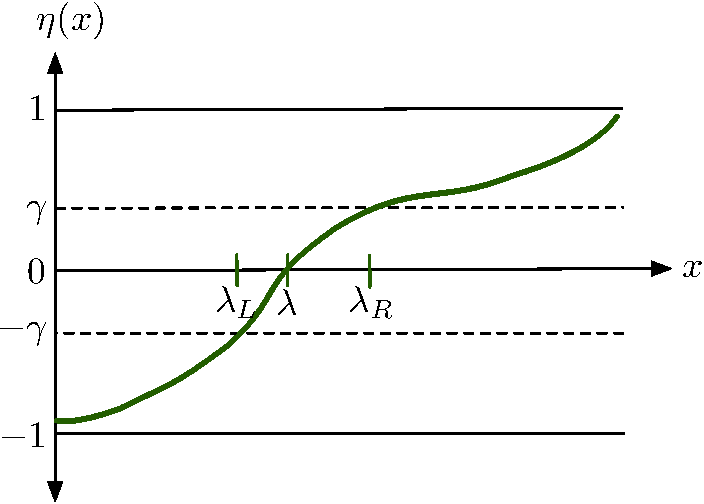
\includegraphics[width=3in]{oned-monotonic.pdf}
\end{center}
\caption{The conditional probability function $\eta$ is monotonically increasing. The values $x = \lambda_L, \lambda, \lambda_R$ have $\eta(x) = -\gamma, 0, \gamma$ respectively.}
\label{fig:oned-monotonic}
\end{figure}


\begin{lemma}
Pick any $x \in [0, \lambda_L] \cup [\lambda_R, 1]$.
\begin{enumerate}
\item[(a)] Define $n^- = |[0,\lambda_L) \cap X|$ and $n^+ = |(\lambda_R,1] \cap X|$. Then
$$
L_s(x)
\leq
\left\{
\begin{array}{ll}
\lg n/n^+ & \mbox{if $x > \lambda_R$} \\
\lg n/n^- & \mbox{if $x < \lambda_L$}
\end{array}
\right.
$$
\item[(b)] Let $r(x)$ be the number of points between $x$ and the boundary point $\lambda$, counting $x$ itself. That is, $r(x) = |[x,\lambda) \cap X|$ if $x < \lambda$, or $|(\lambda, x] \cap X|$ if $x > \lambda$. Then
$$ L_f(x) \leq \max\left( L_s(x), \left\lceil \lg \frac{n}{r(x)} -1 \right\rceil \right).$$
\end{enumerate}
\label{lemma:oned-monotonic-Lsf}
\end{lemma}
\begin{proof}
For (a), take any $x > \lambda_R$ (the other case is similar). The interval $B = (\lambda,1)$ lies in $\B_\ell(x)$ for $\ell = \lceil \lg (n/n^+) - 1 \rceil$ and has $\eta_X(B) > b_2$. For larger $\ell$, we get a similar result with a suitable sub-interval of $(\lambda,1)$.

For (b), note that for $\ell \geq \lceil \lg (n/r(x)) - 1 \rceil$, there is no $B \in \B_\ell(x)$ that extends to the other side of the boundary. Moreover, for $\ell \geq L_s(x)$, there is at least one interval in $\B_\ell(x)$ with bias of the correct sign and magnitude at least $b_2$.
\end{proof}

\section{Label complexity bounds in the distributional setting}

We now turn to a setting where the points $X$ are sampled from a distribution $\mu$ on $\X$. The algorithm is unchanged, but we seek to bound label complexity in terms of properties of the joint distribution specified by $\mu$ and $\eta$.

\subsection{Sampling level and probability mass}

To begin with, we relate the number of points in a ball $B \in \B$ (and thus the level of the ball) to its probability mass under the marginal distribution.
\begin{lemma}
With probability at least $1-\delta$, for all $B \in \B$ with $n \mu(B) \geq 12 \ln (2|\B|/\delta)$, we have
$$ \frac{\mu(B)}{2} \leq \frac{|X_B|}{n} \leq 2 \mu(B) .$$
\label{lemma:ball-size-bounds}
\end{lemma}
\begin{proof}
It is an immediate consequence of the multiplicative Chernoff bound that with probability at least $1-\delta$, for all $B \in \B$,
$$ \frac{|X_B|}{n} = \mu(B) \left(1 \pm \sqrt{\frac{3}{n \mu(B)} \ln \frac{2|\B|}{\delta}} \right) .$$
\end{proof}

Henceforth assume that this high-probability event holds. Now, if $B \in \B_\ell$, then
$$ \mu(B) \leq \frac{2 |X_B|}{n} < \frac{2}{2^\ell} $$
and thus $\ell < \lg (2/\mu(B))$. A similar chain of inequalities in the other direction yields $\ell \geq \lg 1/(4 \mu(B))$. We thus see that balls of probability mass $p$ belong to level $\ell \approx \lg (1/p)$.

\subsection{Adjustments to the finite population analysis}

In the distributional setting, our notion of the \emph{average bias} of a ball $B \in \B$ changes from the quantity $\eta_X(B)$ defined earlier (namely, the average $\eta$-value of the finite set of points $X \cap B$) to
$$ \eta(B) = \frac{1}{\mu(B)} \int \eta \, d\mu ,$$
which is defined as long as $\mu(B) > 0$. Correspondingly, we relate the accuracy of bias estimates $\yh(B)$ to $\eta(B)$ rather than $\eta_X(B)$.
\begin{defn}
For any $B \in \B$ and $0 < b_1 < b_2$, we say bias estimate $\yh(B) \in \{+1,-1,0\}$ is \emph{distributionally $(b_1,b_2)$-accurate} if the following holds:
\begin{itemize}
\item $\yh(B) = +1 \implies \eta(B) > b_1$
\item $\yh(B) = -1 \implies \eta(B) < -b_1$
\item $\yh(B) = 0 \implies |\eta(B)| < b_2$
\end{itemize}
\label{def:accurate-bias-estimate-dist}
\end{defn}

We can show that Theorem~\ref{thm:large-deviation-bounds} and Corollary~\ref{cor:accurate-bias-estimates} continue to hold with $\eta(B)$ in place of $\eta_X(B)$. We state the result here for convenience.
\begin{thm}
Suppose that $k \geq (8c_1/(b_2-b_1))^2$ where $c_1$ is given in (\ref{eq:c1}). 
For each $B \in \B$, let $\widehat{\eta}(B)$ be the average label on the query-set $\Gamma(B) = \{z \in X_B: T_z \leq \tau_\ell\}$, and define the bias-estimate $\yh(B)$ as follows:
$$ \yh(B)
= 
\left\{
\begin{array}{ll}
\sign(\widehat{\eta}(B)) & \mbox{if $|\widehat{\eta}(B)| \geq (b_1 + b_2)/2$} \\
0 & \mbox{otherwise}
\end{array}
\right.
$$
With probability $\geq 1-\delta$, all bias estimates $\yh(B)$, for $B \in \B$, are distributionally $(b_1,b_2)$-accurate.
\label{thm:accurate-bias-estimates-dist}
\end{thm}

We need to make a similar small adjustment to the definitions of $L_s$ and $L_f$, merely swapping $\eta_X(B)$ for $\eta(B)$. Under the modified definitions, Lemma~\ref{lemma:focused} continues to hold; we restate it here for reference.
\begin{lemma}
All focused samples at level $\ell$ lie in $\{z \in \Delta_\ell: T_z \leq \tau_\ell \}$, where
$$ \Delta_\ell = \bigcup_{x \in X: L_f(x) \geq \ell} \bigcup_{B \in \B_{\ell}(x)} X_B .$$
\label{lemma:focused-dist}
\end{lemma}

In a similar vein, we have an analog of Lemma~\ref{lemma:level-distribution} for the distributional setting.
\begin{lemma}
With probability at least $1-2(\ell_o+1)e^{-k/3}$, the following hold for all levels $0 \leq \ell \leq \ell_o$.
\begin{enumerate}
\item[(a)] $|\{x \in X: T_x \leq \tau_\ell\}| \leq 2 n \tau_\ell$.
\item[(b)] If $\mu(\Delta_\ell) \tau_\ell \geq k/n$ then $|\{x \in \Delta_{\ell}: T_x \leq \tau_\ell\}| \leq 2 n \mu(\Delta_\ell) \tau_\ell$.
\end{enumerate}
\label{lemma:level-distribution-dist}
\end{lemma}
\begin{proof} 
  Part (a) is as in Lemma~\ref{lemma:level-distribution-dist}. For (b), pick any subset $S \subset \X$. If $X$ consists of $n$ independent draws from $\mu$, then $|\{x \in S: T_x \leq \tau_\ell\}|$ has a $\mbox{binomial}(n, \mu(S) \tau_\ell)$ distribution with expectation $n \mu(S) \tau_\ell$. The probability that it is more than twice its expected value is, by a multiplicative Chernoff bound, at most $e^{-n \mu(S) \tau_\ell/3}$.
\end{proof}

Theorem~\ref{thm:label-complexity} continues to hold, in the following form. The only change to the proof is to use Lemma~\ref{lemma:level-distribution-dist}(b) in place of Lemma~\ref{lemma:level-distribution}(b).
\begin{thm}
Suppose the active learning algorithm is allowed to make $0 < m \leq n$ queries. Define
$$ \ell_1 = \left\lfloor \lg \frac{m}{32k} \right\rfloor .$$
and let $\ell_2$ be the largest integer such that
$$ \sum_{\ell = \ell_1 + 1}^{\ell_2} 2^\ell \mu(\Delta_{\ell}) \ \leq \ \frac{m}{32k} .$$
Then any point $x \in X$ with $L_s(x) \leq \ell_1$ and $L_f(x) \leq \ell_2$ will have a final label $\yh(x)$ that is correctly set to $g^*(x)$.
\label{thm:label-complexity-dist}
\end{thm}



\pagebreak

\appendix

\section{Technicalities}

\subsection{Large deviation bounds for the discrete setting}

\begin{lemma}[rechecked]
Fix a confidence parameter $0 < \delta < 1$ and a positive integer $k \geq 6 \ln (4/\delta)$. 

Let $x_1, \ldots, x_m$ be any collection of points. Suppose that the labels $Y_i \in \{-1,1\}$ of these points are independent, with $\E Y_i = \eta(x_i)$. Define
$$ \eta_o = \frac{1}{m} \left( \eta(x_1) + \cdots + \eta(x_m) \right) .$$
Now consider the following estimator $Z$ of this quantity:
\begin{itemize}
\item Each $x_i$ is chosen with probability $q > 0$, independently. Let $N$ be the number of selected points.
\item If $N > 0$, the labels $Y_i$ of the selected points are obtained, and $Z$ is their average.
\end{itemize}
If $qm \geq k + \sqrt{6k \ln (4/\delta)}$, with probability at least $1-\delta$, 
\begin{enumerate}
\item[(a)] $N \geq k$, and 
\item[(b)] $| Z - \eta_o| < \sqrt{(48/k) \ln (4/\delta)}$.
\end{enumerate}
\label{lemma:large-deviation-discrete}
\end{lemma}
\begin{proof}
Let's start with (a). Define $c_1 = \sqrt{3 \ln (4/\delta)}$. We'll take $qm = k + \sqrt{6k \ln (4/\delta)} = k + c_1 \sqrt{2k}$ since this is the worst case. By assumption, $k \geq 2c_1^2$ and thus $qm \leq 2k$.

Now, $N$ has a binomial($m,q$) distribution. By a multiplicative Chernoff bound, for $0 < \epsilon < 1$, we have
\begin{align*}
\pr(N \geq qm(1+\epsilon)) &\leq e^{-qm\epsilon^2/3} \\
\pr(N \leq qm(1-\epsilon)) &\leq e^{-qm\epsilon^2/2}
\end{align*}
Take $\epsilon = c_1/\sqrt{qm}$; by the lower bound on $k$, we have $\epsilon \leq 1/2$. Recalling the choice of $c_1$, we see that with probability at least $1-\delta/2$, we get 
$$(1-\epsilon) qm < N < (1+\epsilon) qm .$$
The lower bound implies $N > qm(1-\epsilon) = qm - c_1\sqrt{qm} = k + c_1 \sqrt{2k} - c_1 \sqrt{qm} \geq k$.

For (b), define $C_1, \ldots, C_m \in \{0,1\}$ as random variables indicating whether the corresponding points were selected; that is, $C_i = {\bf 1}(\mbox{$x_i$ was selected})$. The sum of the obtained labels is then $S = C_1 Y_1 + \cdots + C_m Y_m$. Notice that these $C_iY_i \in \{-1,0,1\}$ are independent with $\E[C_iY_i] = q \eta(x_i)$ and $\E[(C_iY_i)^2] = \E[C_i] = q$. Thus their sum $S$ has expectation
$$ \E [S] = \sum_{i=1}^m \E[C_i Y_i] = \sum_{i=1}^m q \eta(x_i) = qm \eta_o $$
and variance
$$ \mbox{var}(S) = \sum_{i=1}^m \mbox{var}(C_iY_i) \leq qm .$$
We can bound the concentration of $S$ around its expected value using Bernstein's inequality, by which
$$ \pr(|S - \E[S]| \geq t) \leq 2 \exp \left( - \frac{t^2}{2(\mbox{var}(S) + t/3)} \right) .$$
Using $t = \epsilon qm$, we then have that $|S - qm \eta_o| \leq \epsilon qm$ with probability at least $1-\delta/2$.

Combining with the high-probability bound on $N$ above, we get
$$ \frac{qm \eta_o - \epsilon qm}{qm(1+\epsilon)} < \frac{S}{N} < \frac{qm \eta_o + \epsilon qm}{qm(1-\epsilon)},$$
whereupon (recalling $Z = S/N$)
$$ 
\eta_o \left( \frac{1}{1+\epsilon} -1 \right) - \frac{\epsilon}{1+\epsilon} < Z - \eta_o < \eta_o \left( \frac{1}{1-\epsilon} - 1 \right) + \frac{\epsilon}{1-\epsilon} .$$
Since $|\eta_o| \leq 1$,
$$ |Z - \eta_o | < \max \left( \frac{2\epsilon}{1+\epsilon}, \frac{2\epsilon}{1-\epsilon} \right)
\leq 
4 \epsilon,$$
as claimed.  
\end{proof}

\subsection{Large deviation bounds for the continuous setting}

Let $\mu$ be a distribution on the instance space $\X$.

\begin{lemma}[checked]
Fix a confidence parameter $0 < \delta < 1$ and a positive integer $k \geq 6 \ln (4/\delta)$. 

Pick a set $B \subset \X$ with $\mu(B) > 0$. Suppose $m$ points $x_1, \ldots, x_m$ are drawn from $\mu|_B$, the restriction of $\mu$ to $B$, and their labels $y_1, \ldots, y_m \in \{-1,+1\}$ are generated according to $\eta$, that is, $\E[Y_i|x_i] = \eta(x_i)$.

Consider the following estimator $Z$ of $\eta(B)$:
\begin{itemize}
\item Each $x_i$ is chosen with probability $q > 0$, independently. Let $N$ be the number of selected points.
\item The labels of the selected points are averaged, yielding a value $Z$ (which defaults to 0 if no points were selected).
\end{itemize}
If $qm \geq k + \sqrt{6k \ln (4/\delta)}$, with probability at least $1-\delta$, 
\begin{enumerate}
\item[(a)] $N \geq k$, and 
\item[(b)] $| Z - \eta(B)| < \sqrt{(48/k) \ln (4/\delta)}$.
\end{enumerate}
\label{lemma:large-deviation-continuous}
\end{lemma}

\begin{proof}
This exactly follows the proof of Lemma~\ref{lemma:large-deviation-discrete}, with $\eta(B)$ in place of $\eta_o$.
\end{proof}

Next, we show that the $\eta_X(B)$ are, in turn, close to the corresponding $\eta(B)$.
\begin{lemma}
Fix any confidence parameter $0 < \delta < 1$. Then with probability at least $1-\delta$, the following holds for all $B \in \B$:
$$ \left| \eta(B) - \eta_X(B) \right| \leq \sqrt{\frac{2}{|X_B|} \ln \frac{2|\B|}{\delta}} .$$
\label{lemma:discrete-to-continuous}
\end{lemma}
\begin{proof}
Pick any $B \in \B$. The points in $X_B$ are random draws from $\mu|_B$. Each such point $Z$ has $\eta(Z) \in [-1,1]$ with $\E[\eta(Z)] = \eta(B)$. By a Hoeffding bound,
$$ \pr(|\eta_X(B) - \eta(B)| \geq t) \leq 2e^{-t^2|X_B|/2} $$
for any $t > 0$. The result follows by taking 
$$t = \sqrt{\frac{2}{|X_B|} \ln \frac{2|\B|}{\delta}}$$ 
and applying a union bound over all $B \in \B$.
\end{proof}


\end{document}
